\documentclass[a4paper,12pt,twoside]{report}
\usepackage[left=2cm,right=2cm,top=2cm,bottom=3cm]{geometry}
\usepackage[greek,english]{babel}
\usepackage{amsmath}
\usepackage{graphicx}
\usepackage{hyperref}
\hypersetup{
    colorlinks=true,
    linkcolor=blue,
    filecolor=blue,
    urlcolor=blue,
}

\newcommand{\submitdate}{\gr{Σεπτέμβριος 2024}}

\newcommand{\gr}{\selectlanguage{greek}}
\newcommand{\en}{\selectlanguage{english}}

\renewcommand{\thesection}{\arabic{section}}

\begin{document}

\begin{titlepage}
    \centering
    \includegraphics[width=0.5\textwidth]{images/ionio.png} 
    \vspace{1cm}
    
    {\huge\bfseries \gr{Αναφορά Εργασίας στην Τεχνολογία Λογισμικού}\par} 
    \vspace{2cm}
    
    {\Large \gr{Όνομα: Κωνσταντίνος Καφτεράνης}\par} 
    \vspace{0.5cm}
    
    {\Large \gr{ΑΜ: \en{inf2021090}}\par} 
    \vfill
    
    {\large \submitdate\par} 
\end{titlepage}

\renewcommand{\contentsname}{\gr{Περιεχόμενα}} 
\tableofcontents

\section{\gr{Εισαγωγή}}

\gr{Για την εργασία του μαθήματος Τεχνολογία Λογισμικού, δημιουργήθηκε μια διαδικτυακή εφαρμογή μηχανικής μάθησης για την ανάλυση δεδομένων. Η υλοποίηση πραγματοποιήθηκε με τη γλώσσα προγραμματισμού} \en{Python} \gr{χρησιμοποιώντας τη βιβλιοθήκη} \en{Streamlit} \gr{καθώς και άλλες βιβλιοθήκες μηχανικής μάθησης όπως} \en{Scikit-learn, Pandas} \gr{και} \en{Matplotlib}. \gr{Η εφαρμογή ενσωματώνει διάφορους αλγορίθμους μηχανικής μάθησης για κατηγοριοποίηση και ομαδοποίηση, ενώ προσφέρει δυνατότητες οπτικοποίησης των δεδομένων μέσω γραφημάτων και διαγραμμάτων. Η εφαρμογή παρέχει μια φιλική προς τον χρήστη διεπαφή για τη φόρτωση δεδομένων, την επεξεργασία τους και την εξαγωγή πολύτιμων πληροφοριών μέσω στατιστικής ανάλυσης και οπτικοποίησης.}

\section{\gr{Μεθοδολογία Υλοποίησης}} 

\subsection{\gr{Μοντέλο Επαναληπτικής Ανάπτυξης}}
\gr{Το Μοντέλο Επαναληπτικής Ανάπτυξης είναι μια ευέλικτη προσέγγιση ανάπτυξης λογισμικού που βασίζεται στη συνεχή βελτίωση του λογισμικού μέσα από επαναλαμβανόμενες φάσεις ανάπτυξης.}
\begin{itemize}
    \item \gr{Ξεκινάει με τη συλλογή των απαιτήσεων και την ανάλυση των αναγκών του έργου.}
    \item \gr{Ο κώδικας γράφεται σε μικρές, διαχειρίσιμες μονάδες, με κάθε μονάδα να δοκιμάζεται ξεχωριστά, δίνοντας έμφαση στη διόρθωση λαθών πριν προχωρήσουμε στην επόμενη ενότητα.}
    \item \gr{Η ανάπτυξη γίνεται τμηματικά, με την ολοκλήρωση κάθε μονάδας να συμβάλλει στη συνολική ανάπτυξη του συστήματος.}
    \item \gr{Οι τελικές διορθώσεις και βελτιώσεις γίνονται μόνο όταν το κύριο σύστημα είναι σταθερό και λειτουργικό.}
\end{itemize}
\gr{Αυτή η προσέγγιση επιτρέπει την γρήγορη διόρθωση λαθών και την καλύτερη διαχείριση των απαιτήσεων που μπορεί να αλλάζουν κατά την ανάπτυξη της εφαρμογής.}

\section{\gr{Δομή Εφαρμογής}} 

\begin{figure}[h]
    \centering
    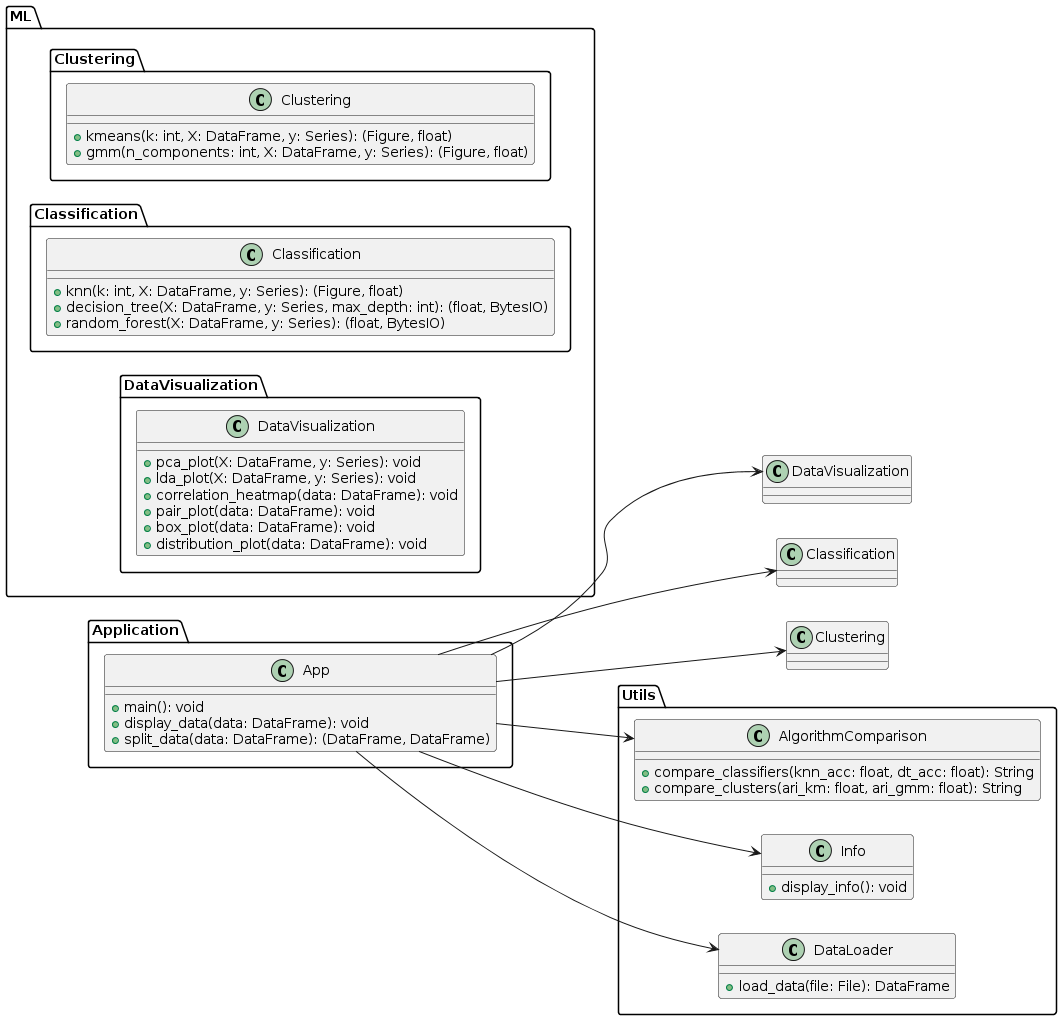
\includegraphics[width=0.6\textwidth]{diagram/diagram.png} 
    \caption{\gr{Το} \en{UML} \gr{διάγραμμα.}}
%    \label{fig:my_figure} % Optional: 
\end{figure}

\subsection{\en{ML}}
\subsection{\en{Utils}}
\subsection{\en{App}}

\section{\gr{Παρουσίαση Εφαρμογής}}

\gr{Παρακάτω εξηγείται πώς χρησιμοποιούμε την εφαρμογή. Κατά την είσοδο στην εφαρμογή, ο χρήστης έρχεται σε επαφή με το UI, το οποίο περιλαμβάνει ένα widget για ανέβασμα αρχείων, καθώς και ένα sidebar menu που χρησιμοποιεί για να περιηγηθεί στην εφαρμογή.}

% Εικόνα για Οθόνη Έναρξης
\begin{figure}[htbp]
    \centering
    \includegraphics[width=0.8\textwidth]{images/opening.png} 
    \caption{\gr{Οθόνη Έναρξης}}
    \label{fig:opening_screen}
\end{figure}

% Εικόνα για Μενού
\begin{figure}[htbp]
    \centering
    \includegraphics[width=0.8\textwidth]{images/menu.png} 
    \caption{\gr{Μενού}}
    \label{fig:menu}
\end{figure}

\gr{Τα αρχεία δεδομένων πρέπει να είναι της μορφής} \en{Excel} \gr{ή} \en{CSV}\gr{, αλλιώς η εφαρμογή δεν θα επιτρέψει το ανέβασμά τους και θα ζητήσει από τον χρήστη να τα ανεβάσει ξανά.}

% Εικόνα για Φόρτωση Δεδομένων
\begin{figure}[htbp]
    \centering
    \includegraphics[width=0.8\textwidth]{images/data.png}
    \caption{\gr{Φόρτωση Δεδομένων}}
    \label{fig:data_loading}
\end{figure}

\gr{Αφού το αρχείο ανέβει, εμφανίζονται τα δεδομένα χωρισμένα σε χαρακτηριστικά} (\en{features}) \gr{και ετικέτες.}

% Δεδομένa
\begin{figure}[htbp]
    \centering
    \includegraphics[width=0.8\textwidth]{images/data.png}
    \caption{\gr{Δεδομένα}}
    \label{fig:data}
\end{figure}

\gr{Στο μενού, ο χρήστης μπορεί να επιλέξει την επεξεργασία που θα εφαρμόσει στα δεδομένα: οπτικοποίηση, εφαρμογή μηχανικής μάθησης ή τη σελίδα με τις οδηγίες.}

\gr{Αν επιστρέψει στο ανέβασμα αρχείων, τότε τα δεδομένα χάνονται και ζητείται να ανέβει ένα καινούργιο αρχείο.}


\gr{Επιλέγοντας οπτικοποίηση, ο χρήστης έχει δύο δυνατότητες. Από ένα} \en{dropdown menu} \gr{επιλέγει είτε τον αλγόριθμο} \en{PCA} \gr{ή} \en{LDA} \gr{και να δημιουργήσει ένα διάγραμμα, καθώς επίσης και μερικά διαγράμματα επεξηγηματικών δεδομένων, τα οποία θα εμφανιστούν κάθετα κάτω από το διάγραμμα του αλγορίθμου οπτικοποίησης. Τα διαγράμματα αυτά είναι:}

% Εικόνα για Οπτικοποίηση Δεδομένων
\begin{figure}[htbp]
    \centering
    \includegraphics[width=0.8\textwidth]{images/vizualization.png} 
    \caption{\gr{Οπτικοποίηση Δεδομένων}}
    \label{fig:data_visualization}
\end{figure}


\begin{figure}[htbp]
    \centering
    \includegraphics[width=0.8\textwidth]{images/lda.png} 
    \caption{\gr{Ο αλγόριθμος \en{LDA}}}
    \label{fig:data_visualization_lda}
\end{figure}
\gr{Όσον αφορά τη μηχανική μάθηση, ο χρήστης μπορεί να επιλέξει ανάμεσα σε δύο προβλήματα,} \en{classification} \gr{και} \en{clustering}\gr{, τσεκάροντας το αντίστοιχο κυκλάκι. Στην περίπτωση της κατηγοριοποίησης, ο χρήστης επιλέγει μεταξύ των αλγορίθμων} \en{k-means} \gr{και} \en{decision tree}\gr{. Σε κάθε περίπτωση, χρησιμοποιεί μια μπάρα για να επιλέξει το} \en{k}\gr{, και εφαρμόζονται και οι δύο αλγόριθμοι. Τα αποτελέσματα συγκρίνονται με βάση τον δείκτη} \en{accuracy} \gr{για να αξιολογηθεί η επίδοσή τους. Τις περισσότερες φορές, το} \en{decision tree} \gr{υπερέχει του} \en{k-nearest neighbors (KNN)}\gr{, καθώς για μερικές τιμές του} \en{k} \gr{το} \en{KNN} \gr{υπερπροσαρμόζεται} (\en{overfits})\gr{. Εμφανίζεται μήνυμα που προειδοποιεί τον χρήστη να επιλέξει τον κατάλληλο αλγόριθμο κάθε φορά.}

\begin{figure}[htbp]
    \centering
    \includegraphics[width=0.8\textwidth]{images/tree.png} 
    \caption{\gr{Δ'εντρο Επιλογής}}
    \label{fig:tree}
\end{figure}

\begin{figure}[htbp]
    \centering
    \includegraphics[width=0.8\textwidth]{images/overfits.png} 
    \caption{\gr{Υπερπροσαρμογή}}
    \label{fig:overfits}
\end{figure}

\gr{Όσον αφορά το} \en{clustering}\gr{, ο χρήστης μπορεί να επιλέξει μεταξύ των αλγορίθμων} \en{Gaussian Mixture Model (GMM)} \gr{και} \en{k-means}\gr{. Κανένας από τους δύο αλγορίθμους δεν υπερπροσαρμόζεται} (\en{overfits})\gr{, αλλά η απόδοσή τους μπορεί να διαφέρει ανάλογα με τα δεδομένα. Σε ορισμένες περιπτώσεις, το} \en{GMM} \gr{αποδίδει καλύτερα, ενώ σε άλλες το} \en{k-means} \gr{είναι πιο αποδοτικό. Για τη σύγκριση των αποτελεσμάτων χρησιμοποιείται ο δείκτης} \en{Adjusted Rand Index (ARI)}\gr{, ο οποίος επιτρέπει την αξιολόγηση της ποιότητας των ομάδων που δημιουργούνται από κάθε αλγόριθμο.}

\begin{figure}[htbp]
    \centering
    \includegraphics[width=0.8\textwidth]{images/clustering.png} 
    \caption{\en{Clustering}}
    \label{fig:clustering}
\end{figure}

\section{\gr{Χρήση μέσω }\en{Docker}}

\begin{itemize}
    \item \gr{Η εικόνα} \en{Python 3.9 Slim} \gr{χρησιμοποιείται ως βάση.}
    \item \en{Working directory to} \texttt{/app}.
    \item \gr{Αντιγράφει το αρχείο} \en{requirements.txt} \gr{στο κοντέινερ.}
    \item \gr{Κατεβάζει τα πακέτα από} \en{requirements.txt} \en{χωρις} \gr{caching.}
    \item \gr{Αντιγράφει τον φάκελο} \en{src/} \gr{στο κοντέινερ.}
    \item \en{Exposes port 8501 for the app.}
    \item \gr{Η εντολή} \en{CMD} \gr{τρέχει την εφαρμογή} \en{Streamlit} \gr{στην πόρτα 8501, ώστε να είναι προσβάσιμη.}
\end{itemize}


\gr{Για την ανάπτυξη και διανομή της εφαρμογής:}
\begin{itemize}
    \item \gr{Εκτελέστε την εντολή} \en{\ \texttt{docker build -t my-streamlit-app .}} \gr{για να δημιουργήσετε την εικόνα.}
    \item \gr{Εκτελέστε την εντολή} \en{\ \texttt{docker run -p 8501:8501 my-streamlit-app}} \gr{για να τρέξετε την εφαρμογή στη διεύθυνση} \en{\ \texttt{http://localhost:8501}}.
\end{itemize}
\section{\gr{Ομάδα}}
\section{\gr{Κώδικας}}

\begin{itemize}
    \item \en{\href{https://github.com/inf2021090/sw-project}{Project GitHub Repository}} 
    \item \en{\href{https://github.com/inf2021090}{GitHub Profile}} 
    \item \en{\href{https://github.com/inf2021090/sw-project/tree/main/src}{Source Code}} 
    \item \en{\href{https://github.com/your-repo/raw-latex-file.tex}{Report Raw LaTeX File}} 
    \item \en{\href{https://github.com/your-repo/report.pdf}{Report PDF}} 
    \item \en{\href{https://github.com/inf2021090/sw-project/blob/main/docs/diagram/diagram.png}{UML Diagram}} 
\end{itemize}

\end{document}
